\documentclass[11pt]{article}

\usepackage[margin=1in]{geometry}
\usepackage{amsmath, amssymb}
\usepackage{booktabs}
\usepackage{enumitem}
\usepackage{hyperref}
\usepackage{tikz}
\usetikzlibrary{arrows.meta, positioning, shapes.geometric}

\title{Junction Wearables Reliability Project:\\Version 1, Version 2, and Reframed Scope}
\author{Keval Amin}
\date{\today}

\tikzset{
  box/.style={
    rectangle,
    rounded corners,
    draw=black,
    align=center,
    minimum width=2.7cm,
    minimum height=0.9cm
  },
  decision/.style={
    diamond,
    draw=black,
    align=center,
    aspect=2,
    inner sep=1pt
  },
  arrow/.style={
    -{Latex[length=2.5mm]},
    thick
  }
}

\begin{document}

\maketitle

\section{Executive Summary}

This project studies a Junction-style product question:
\begin{quote}
When should a wearable-derived recovery signal be surfaced confidently, surfaced with warning, or suppressed?
\end{quote}

The project has two versions.

\begin{itemize}[leftmargin=1.5em]
    \item \textbf{Version 1} is a heuristic confidence-policy pipeline. It converts wearable coverage and consistency features into a hand-built reliability score and then maps that score to a product action.
    \item \textbf{Version 2} is a learned reliability-model pipeline. It uses paired early and mature snapshots to predict whether an early signal is likely to remain stable after backfill, and uses IPW/AIPW to correct evaluation under selective label observability.
\end{itemize}

The key reframing is important:
\begin{quote}
This repository currently supports a \textbf{signal surfacing and stability} claim, not a full \textbf{physiological or clinical validity} claim.
\end{quote}

\section{Why This Project Exists}

Junction's value is not just normalization of wearable data into a consistent schema. A downstream product still needs to decide whether a score is reliable enough to act on. Health and wearable data are often sparse, noisy, inconsistent across providers, and subject to backfill.

This project focuses on the reliability layer between:
\begin{enumerate}[leftmargin=1.5em]
    \item standardized data ingestion, and
    \item decision-grade product behavior.
\end{enumerate}

\section{Version 1 Overview}

Version 1 is a heuristic reliability policy. It ingests standardized sleep summaries, builds daily provider-level features, computes a confidence score, and maps the score into a user-facing recommendation.

\subsection{Version 1 Flow}

\begin{center}
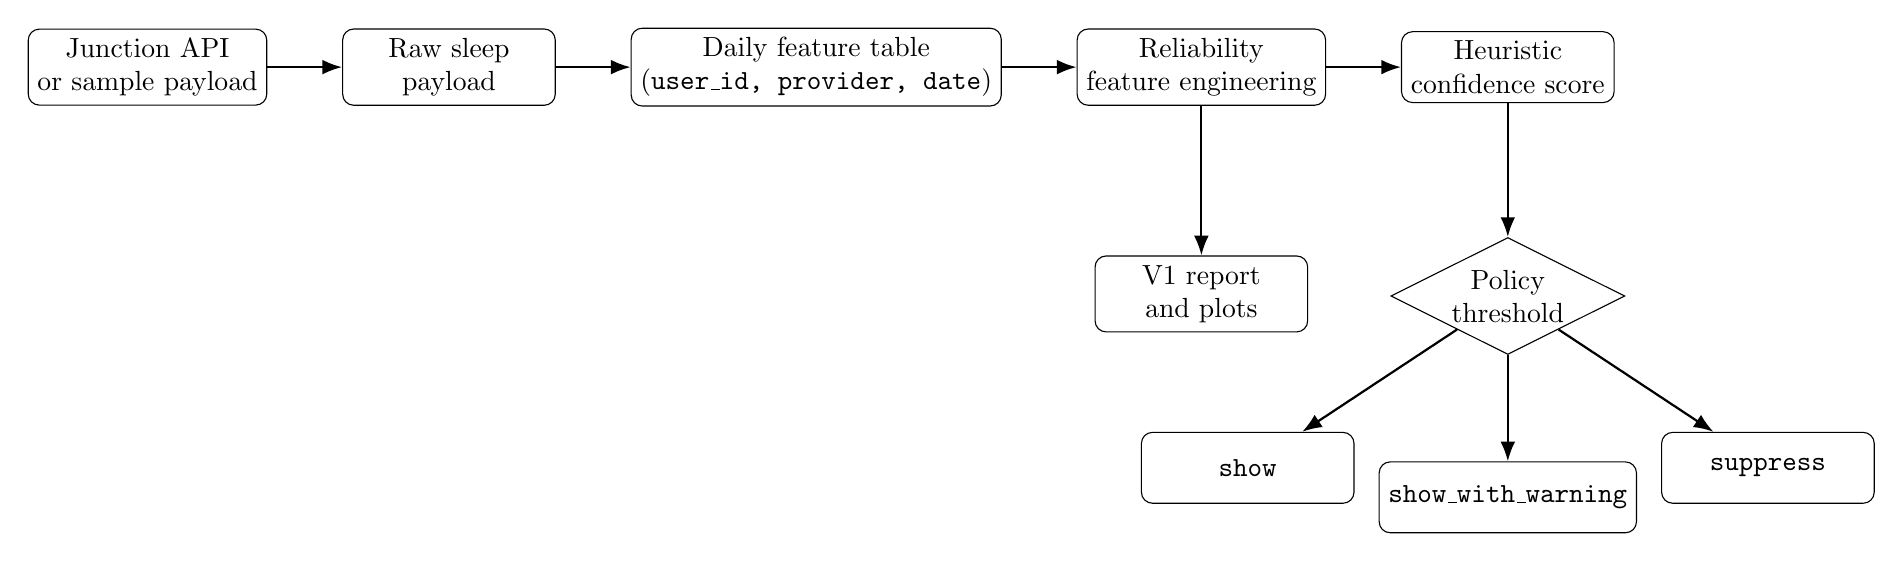
\begin{tikzpicture}[node distance=1.55cm and 0.95cm]
    \node[box] (api) {Junction API\\or sample payload};
    \node[box, right=of api] (raw) {Raw sleep\\payload};
    \node[box, right=of raw] (features) {Daily feature table\\(\texttt{user\_id, provider, date})};
    \node[box, right=of features] (eng) {Reliability\\feature engineering};
    \node[box, right=of eng] (score) {Heuristic\\confidence score};
    \node[decision, below=1.7cm of score] (policy) {Policy\\threshold};
    \node[box, below left=1.35cm and 1.2cm of policy] (show) {\texttt{show}};
    \node[box, below=1.35cm of policy] (warn) {\texttt{show\_with\_warning}};
    \node[box, below right=1.35cm and 1.2cm of policy] (suppress) {\texttt{suppress}};
    \node[box, below=1.9cm of eng] (reportv1) {V1 report\\and plots};

    \draw[arrow] (api) -- (raw);
    \draw[arrow] (raw) -- (features);
    \draw[arrow] (features) -- (eng);
    \draw[arrow] (eng) -- (score);
    \draw[arrow] (score) -- (policy);
    \draw[arrow] (policy) -- (show);
    \draw[arrow] (policy) -- (warn);
    \draw[arrow] (policy) -- (suppress);
    \draw[arrow] (eng) -- (reportv1);
\end{tikzpicture}
\end{center}

\subsection{Version 1 Features}

Version 1 uses interpretable inputs such as:
\begin{itemize}[leftmargin=1.5em]
    \item recent completeness over the last 7 days,
    \item backfill completeness over the requested window,
    \item number of baseline nights in the last 28 days,
    \item stability relative to recent history,
    \item provider agreement when multiple sources overlap.
\end{itemize}

\subsection{Version 1 Math}

The Version 1 confidence score is:
\[
\text{confidence}_i
=
0.35 \cdot c_{7d,i}
+ 0.25 \cdot b_i
+ 0.20 \cdot n_i
+ 0.10 \cdot s_i
+ 0.10 \cdot a_i,
\]
where:
\begin{itemize}[leftmargin=1.5em]
    \item $c_{7d,i}$ is 7-day completeness,
    \item $b_i$ is backfill completeness,
    \item $n_i$ is normalized baseline sufficiency,
    \item $s_i$ is a stability score,
    \item $a_i$ is a provider agreement score.
\end{itemize}

The decision policy is:
\begin{align*}
\texttt{show} &\quad \text{if confidence} \ge 0.75, \\
\texttt{show\_with\_warning} &\quad \text{if } 0.50 \le \text{confidence} < 0.75, \\
\texttt{suppress} &\quad \text{if confidence} < 0.50.
\end{align*}

\subsection{Version 1 Strengths}

\begin{itemize}[leftmargin=1.5em]
    \item It is easy to explain.
    \item It maps directly to a product policy.
    \item It is conservative under sparse or contradictory data.
    \item It demonstrates good feature engineering on messy wearable data.
\end{itemize}

\subsection{Version 1 Limitations}

\begin{itemize}[leftmargin=1.5em]
    \item The weights are heuristic rather than learned.
    \item The thresholds are product choices rather than calibrated estimates.
    \item It does not define an explicit target outcome.
\end{itemize}

\section{Version 2 Overview}

Version 2 extends the project into a supervised learning problem. Instead of assigning weights directly, it asks whether an \emph{early} signal remains close to a later \emph{mature} signal after more backfill has arrived.

\subsection{Version 2 Flow}

\begin{center}
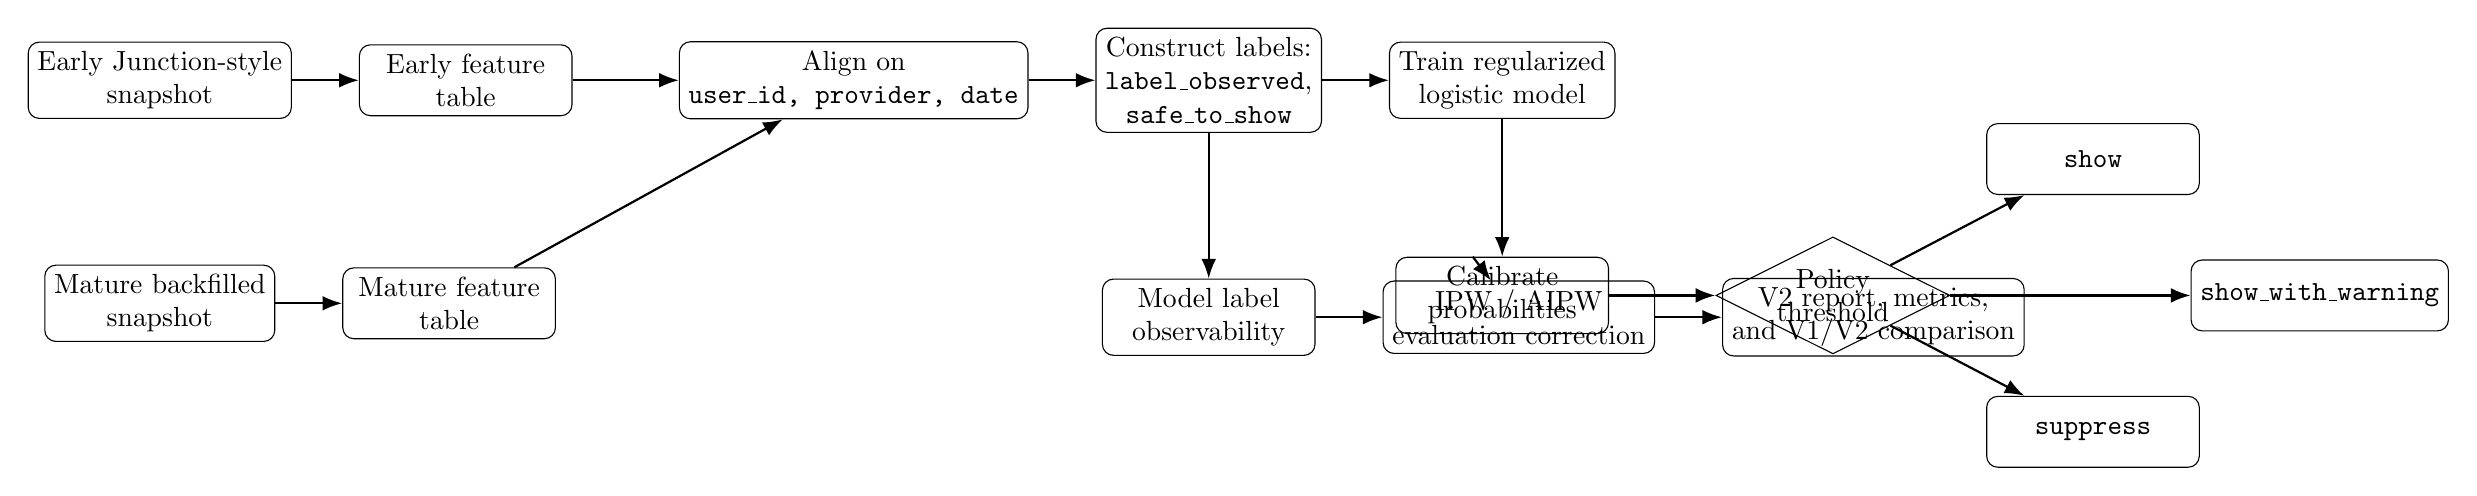
\begin{tikzpicture}[node distance=1.45cm and 0.85cm]
    \node[box] (earlyraw) {Early Junction-style\\snapshot};
    \node[box, right=of earlyraw] (earlyft) {Early feature\\table};
    \node[box, below=1.85cm of earlyraw] (matureraw) {Mature backfilled\\snapshot};
    \node[box, right=of matureraw] (matureft) {Mature feature\\table};
    \node[box, right=of earlyft, xshift=0.5cm] (align) {Align on\\\texttt{user\_id, provider, date}};
    \node[box, right=of align] (label) {Construct labels:\\\texttt{label\_observed},\\\texttt{safe\_to\_show}};
    \node[box, right=of label] (model) {Train regularized\\logistic model};
    \node[box, below=1.75cm of model] (cal) {Calibrate\\probabilities};
    \node[decision, right=of cal, xshift=0.5cm] (policy2) {Policy\\threshold};
    \node[box, above right=0.9cm and 1.2cm of policy2] (show2) {\texttt{show}};
    \node[box, right=of policy2, xshift=2.2cm] (warn2) {\texttt{show\_with\_warning}};
    \node[box, below right=0.9cm and 1.2cm of policy2] (suppress2) {\texttt{suppress}};
    \node[box, below=1.85cm of label] (prop) {Model label\\observability};
    \node[box, right=of prop] (ipw) {IPW / AIPW\\evaluation correction};
    \node[box, right=of ipw] (report2) {V2 report, metrics,\\and V1/V2 comparison};

    \draw[arrow] (earlyraw) -- (earlyft);
    \draw[arrow] (matureraw) -- (matureft);
    \draw[arrow] (earlyft) -- (align);
    \draw[arrow] (matureft) -- (align);
    \draw[arrow] (align) -- (label);
    \draw[arrow] (label) -- (model);
    \draw[arrow] (model) -- (cal);
    \draw[arrow] (cal) -- (policy2);
    \draw[arrow] (policy2) -- (show2);
    \draw[arrow] (policy2) -- (warn2);
    \draw[arrow] (policy2) -- (suppress2);
    \draw[arrow] (label) -- (prop);
    \draw[arrow] (prop) -- (ipw);
    \draw[arrow] (cal) -- (ipw);
    \draw[arrow] (ipw) -- (report2);
\end{tikzpicture}
\end{center}

\subsection{Version 2 Label Construction}

For each row $i$, let:
\[
L_i = \mathbf{1}(\text{the mature row exists later with a usable core signal}).
\]

This is \texttt{label\_observed}. The target is only defined when $L_i = 1$.

If both early and mature rows contain a recovery readiness score:
\[
Y_i = 1
\quad \text{if } \left|R_i^{\text{early}} - R_i^{\text{mature}}\right| \le 5.
\]

Otherwise, if the pipeline falls back to average HRV:
\[
Y_i = 1
\quad \text{if }
\left|H_i^{\text{early}} - H_i^{\text{mature}}\right|
\le
\max\left(5,\;0.15|H_i^{\text{mature}}|\right).
\]

If both early and mature sleep efficiency values exist, the project also requires:
\[
\left|S_i^{\text{early}} - S_i^{\text{mature}}\right| \le 5.
\]

If the consistency checks fail, then $Y_i = 0$.

\subsection{Version 2 Predictive Model}

Let $X_i$ denote the feature vector for row $i$. The model is logistic regression:
\[
\hat{p}_i = P(Y_i = 1 \mid X_i)
= \sigma\left(\beta_0 + X_i^\top \beta\right),
\]
where
\[
\sigma(z) = \frac{1}{1+e^{-z}}.
\]

The inputs include:
\begin{itemize}[leftmargin=1.5em]
    \item completeness,
    \item backfill coverage,
    \item baseline nights,
    \item stability score,
    \item leave-one-out provider agreement,
    \item whether the core signal is available,
    \item whether the row uses readiness score or HRV fallback,
    \item provider and source-type indicators,
    \item row-level physiological and sleep summary values.
\end{itemize}

\subsection{Version 2 Calibration and Policy}

The raw model probability is optionally calibrated:
\[
\hat{p}_i^{\,\text{cal}} = g(\hat{p}_i).
\]

The calibrated probability is mapped into the same three product actions:
\begin{align*}
\texttt{show} &\quad \text{if } \hat{p}_i^{\,\text{cal}} \ge 0.75, \\
\texttt{show\_with\_warning} &\quad \text{if } 0.50 \le \hat{p}_i^{\,\text{cal}} < 0.75, \\
\texttt{suppress} &\quad \text{if } \hat{p}_i^{\,\text{cal}} < 0.50.
\end{align*}

\section{Selective Label Observability}

Not every early row later becomes verifiable. That means evaluation on the labeled subset may be biased.

Version 2 models the probability that the label is observed:
\[
\pi(X_i) = P(L_i = 1 \mid X_i).
\]

For labeled rows, the inverse probability weight is:
\[
w_i = \frac{1}{\pi(X_i)}.
\]

These weights are used to compute corrected evaluation metrics.

\subsection{IPW Metric Example}

The weighted Brier score is:
\[
\text{Brier}_{\text{IPW}}
=
\frac{\sum_i w_i \left(Y_i - \hat{p}_i^{\,\text{cal}}\right)^2}{\sum_i w_i}.
\]

\subsection{AIPW Summary}

Let:
\begin{itemize}[leftmargin=1.5em]
    \item $q_i = \hat{p}_i^{\,\text{cal}}$,
    \item $\pi_i = \pi(X_i)$,
    \item $L_i$ indicate whether the label is observed.
\end{itemize}

Then the AIPW-style pseudo-outcome is:
\[
\phi_i = q_i + \frac{L_i}{\pi_i}(Y_i - q_i).
\]

An estimated mean safe-to-show rate is:
\[
\hat{\mu}_{\text{AIPW}} = \frac{1}{n}\sum_{i=1}^n \phi_i.
\]

\section{What the Project Currently Proves}

The current project is strongest when framed as:
\begin{quote}
Can a product decide whether a wearable-derived recovery signal is stable and mature enough to surface?
\end{quote}

That is a valuable and realistic question for a company like Junction. It combines:
\begin{itemize}[leftmargin=1.5em]
    \item messy wearable data,
    \item feature engineering,
    \item uncertainty-aware policy design,
    \item calibrated prediction,
    \item and selective-observability correction.
\end{itemize}

\section{What the Project Does Not Yet Prove}

The key limitation is conceptual:
\begin{quote}
The Version 2 target measures \textbf{stability under backfill}, not \textbf{physiological truth}.
\end{quote}

That means:
\begin{itemize}[leftmargin=1.5em]
    \item a signal can be stable but not clinically meaningful,
    \item a score can survive backfill but still fail to reflect real recovery state,
    \item this repository is not yet a clinical validation study.
\end{itemize}

\section{Why the Reframing Matters}

Earlier wording risked making the project sound like a broader validation claim than it really is. The honest and strongest framing is:
\begin{quote}
This is a reliability and surfacing project, not a completed physiological validation project.
\end{quote}

That distinction is useful in interviews because it shows restraint and good judgment. It says:
\begin{itemize}[leftmargin=1.5em]
    \item I understand uncertainty,
    \item I know the difference between product reliability and clinical truth,
    \item I am not overclaiming from limited data.
\end{itemize}

\section{Role of MMASH}

MMASH is best used as empirical grounding for why this problem matters. It supports the claim that:
\begin{itemize}[leftmargin=1.5em]
    \item HRV-derived recovery proxies can be noisy,
    \item measurement error can distort small relationships,
    \item confidence penalties for sparse or unstable data are justified.
\end{itemize}

It should not be used to imply that the current Junction-style score is already clinically validated.

\section{Strengths}

\begin{enumerate}[leftmargin=1.5em]
    \item \textbf{Strong product framing.} The output is not just a metric; it is a usable action policy.
    \item \textbf{Interpretability.} Both Version 1 and Version 2 are explainable to technical and product stakeholders.
    \item \textbf{Methodological maturity.} IPW and AIPW are used in an appropriate way rather than as decorative causal language.
    \item \textbf{Reproducibility.} The repo supports archived iterations, reports, and explicit versioning.
    \item \textbf{Good judgment under noisy health data.} The project is conservative rather than overconfident.
\end{enumerate}

\section{Limitations}

\begin{enumerate}[leftmargin=1.5em]
    \item \textbf{Proxy target.} Version 2 predicts stability, not health truth.
    \item \textbf{Small live sample size.} The live Junction sandbox data are not yet rich enough for strong empirical claims.
    \item \textbf{Selection assumptions.} IPW/AIPW still depend on observability being sufficiently modeled from observed features.
    \item \textbf{Threshold dependence.} The final action cutoffs remain policy choices.
    \item \textbf{No direct outcome validation yet.} The project does not yet tie the score to downstream physiological or clinical endpoints.
\end{enumerate}

\section{Best Interview Positioning}

A concise and accurate way to present the project is:
\begin{quote}
I built a Junction-style reliability layer for wearable recovery signals. Version 1 encoded interpretable product priors into a confidence policy. Version 2 turned that into a learned model of whether an early signal would remain stable after backfill, then used IPW and AIPW to correct evaluation because only some rows become verifiable later. The project is best understood as a decision-grade surfacing and stability framework rather than a completed clinical validation study.
\end{quote}

\section{Next Step}

The natural Version 3 extension would be to connect the label to a more physiologically grounded outcome, such as:
\begin{itemize}[leftmargin=1.5em]
    \item sleep efficiency,
    \item perceived stress,
    \item questionnaire-based state measures,
    \item or some other external outcome of recovery quality.
\end{itemize}

That would move the project from:
\begin{quote}
Will this signal remain stable after backfill?
\end{quote}
to:
\begin{quote}
Does this signal reflect meaningful recovery information?
\end{quote}

\section{Conclusion}

This repository is a strong applied data science portfolio piece because it shows the full stack of judgment:
\begin{itemize}[leftmargin=1.5em]
    \item data ingestion and normalization,
    \item reliability feature engineering,
    \item interpretable scoring,
    \item supervised modeling,
    \item selective-observability correction,
    \item and product-facing decision design.
\end{itemize}

Its strongest honest claim is not that it has solved recovery physiology. Its strongest claim is that it defines a careful, rigorous framework for deciding when a wearable-derived recovery signal is stable enough to trust in product.

\end{document}
